%%%%%%%%%%%%%%%%%%%%%%%%%%%%%%%%%%%%%%%%%
% Stylish Article
% LaTeX Template
% Version 2.0 (13/4/14)
%
% This template has been downloaded from:
% http://www.LaTeXTemplates.com
%
% Original author:
% Mathias Legrand (legrand.mathias@gmail.com)
%
% License:
% CC BY-NC-SA 3.0 (http://creativecommons.org/licenses/by-nc-sa/3.0/)
%
%%%%%%%%%%%%%%%%%%%%%%%%%%%%%%%%%%%%%%%%%

%----------------------------------------------------------------------------------------
%	PACKAGES AND OTHER DOCUMENT CONFIGURATIONS
%----------------------------------------------------------------------------------------

\documentclass[fleqn,10pt]{SelfArx} % Document font size and equations flushed left

\usepackage{listings} % Required to insert dummy text. To be removed otherwise
\usepackage[titletoc]{appendix}


\lstset{numberstyle=\tiny,numbersep=5pt,language=Lisp,
  stringstyle=\ttfamily\small,basicstyle=\ttfamily\footnotesize,
  showstringspaces=false,breaklines}

%----------------------------------------------------------------------------------------
%	COLUMNS
%----------------------------------------------------------------------------------------

\setlength{\columnsep}{0.55cm} % Distance between the two columns of text
\setlength{\fboxrule}{0.75pt} % Width of the border around the abstract

%----------------------------------------------------------------------------------------
%	COLORS
%----------------------------------------------------------------------------------------

\definecolor{color1}{RGB}{0, 0, 0} % Color of the article title and sections
\definecolor{color2}{RGB}{0,20,20} % Color of the boxes behind the abstract and headings

%----------------------------------------------------------------------------------------
%	HYPERLINKS
%----------------------------------------------------------------------------------------

\usepackage{hyperref} % Required for hyperlinks
\hypersetup{hidelinks,colorlinks,breaklinks=true,urlcolor=color2,citecolor=color1,linkcolor=color1,bookmarksopen=false,pdftitle={Title},pdfauthor={Author}}

%----------------------------------------------------------------------------------------
%	ARTICLE INFORMATION
%----------------------------------------------------------------------------------------

\JournalInfo{CS389R Recursion and Induction, UT Austin, 2015} % Journal information
\Archive{Dr. Warren Hunt, T.A. Dr. Nathan Wetzler} % Additional notes (e.g. copyright, DOI, review/research article)

\PaperTitle{ACL2: Modeling Adders (and other circuits)} % Article title

\Authors{Cole Stewart\textsuperscript{1}} % Authors
\affiliation{\textsuperscript{1}\textit{Department of Computer Science, University of Texas at Austin}} % Author affiliation

\Keywords{ACL2 -- Circuits -- Verification -- Modeling} % Keywords - if you don't want any simply remove all the text between the curly brackets
\newcommand{\keywordname}{Keywords} % Defines the keywords heading name

%----------------------------------------------------------------------------------------
%	ABSTRACT
%----------------------------------------------------------------------------------------

\Abstract{Discusses different variations of modeling and verification of simple circuits
in ACL2. In particular, a method of converting a circuit diagram to a verifiable ACL2
model is discussed, and a lookahead adder from the Texas Instruments TTL vol. 3 is modeled
and verified.}

%----------------------------------------------------------------------------------------

\begin{document}

\flushbottom % Makes all text pages the same height

\maketitle % Print the title and abstract box

\tableofcontents % Print the contents section

\thispagestyle{empty} % Removes page numbering from the first page

%----------------------------------------------------------------------------------------
%	ARTICLE CONTENTS
%----------------------------------------------------------------------------------------

\section*{Introduction} % The \section*{} command stops section numbering

\addcontentsline{toc}{section}{Introduction} % Adds this section to the table of contents
Formalization and verification of circuit outputs has been a necessary task since the 
introduction of computing. In the beginning, there were no formal verification tools available 
to automate that process either. ACL2 offers a first-order logic and programming language
where systems can be modeled and verified in an automated way. Circuits, in particular, can 
be modeled and logically represented differently. 
This project aimed to accomplish 5 goals:

\begin{enumerate}

\item Creation of a Java tool for generating ACL2 models from circuits defined in CEDAR Logic Simulator, which we call CircuitToAcl2
\item Use of tool to generate ACL2 models for each module in CEDAR Logic Simulator and verify correctness
\item Prove correctness of carry-lookahead adder as defined by the f74181 and f74182 in the Texas Instruments TTL
with the use of binary decision diagrams (BDD), unlabeled binary decision diagrams (UBDD), and different
physical model representations. 
\end{enumerate}

%------------------------------------------------

\section{Generating ACL2 Models}
CEDAR Logic Simulator is a software simulator for circuits involving logic gates and other logical modules such as full adders and registers that is often used in teaching computer engineering courses. In the beginning of the project, other tools such as LogiSim were examined as possible arguments to a model conversion application, but no tool seemed to represent the inherent graph in a meaningful way as well as CEDAR. All the tools which were examined used XML for output.

Generating ACL2 models from CEDAR Logic Simulator was slightly more difficult than was originally anticipated. The XML which was output by CEDAR was malformed in some sections and had to be preprocessed and modified to be well-formed XML before being fed into the XML parser. Being careful not to integrate the generator with one specific metamodel was also a bit of a challenge. The most difficult part of the process, however, was ensuring a gate never came after another gate which depended on it in the ACL2 let* expression output by the application. Solving this problem involved performing a graph traversal through the circuit starting at the inputs. Performing this traversal also allowed a cycle detection to be performed simultaneously. Although the framework is general enough to support the creation of other models in ACL2, in the end I only ended up supporting one model. This kept me from spending too much time in Java and allowed me more time to focus on work done in ACL2 alone. The model I ended up supporting is that of a simple netlist. No cycles are allowed in the circuit, as no state is allowed. The output of a circuit using this model is computed by overloading ACL2 functions to perform our bidding.

\subsection{Warming Up}
\subsubsection{Creating a Model of a 4-bit Comparator}
CEDAR has a library of modules which are essentially small circuits composed of gates which can be connected alongside other gates. One such module in the library was a 4-bit comparator. As a simple example, I first modeled the comparator to get warmed up to the process of defining and verifying correctness of circuits in ACL2. In figure 1 a screenshot of CEDAR Logic is shown which contains a simple comparator with 3 outputs: $a>b$, $a<b$, and $a=b$. The ACL2 function in Appendix A shows the output of CircuitToAcl2 with input defined by the circuit in Figure 1.

\begin{figure}[ht!]
  \caption{A 4-bit comparator in CEDAR Logic Simulator}
  {%
\setlength{\fboxsep}{0pt}%
\setlength{\fboxrule}{1pt}%
\fbox{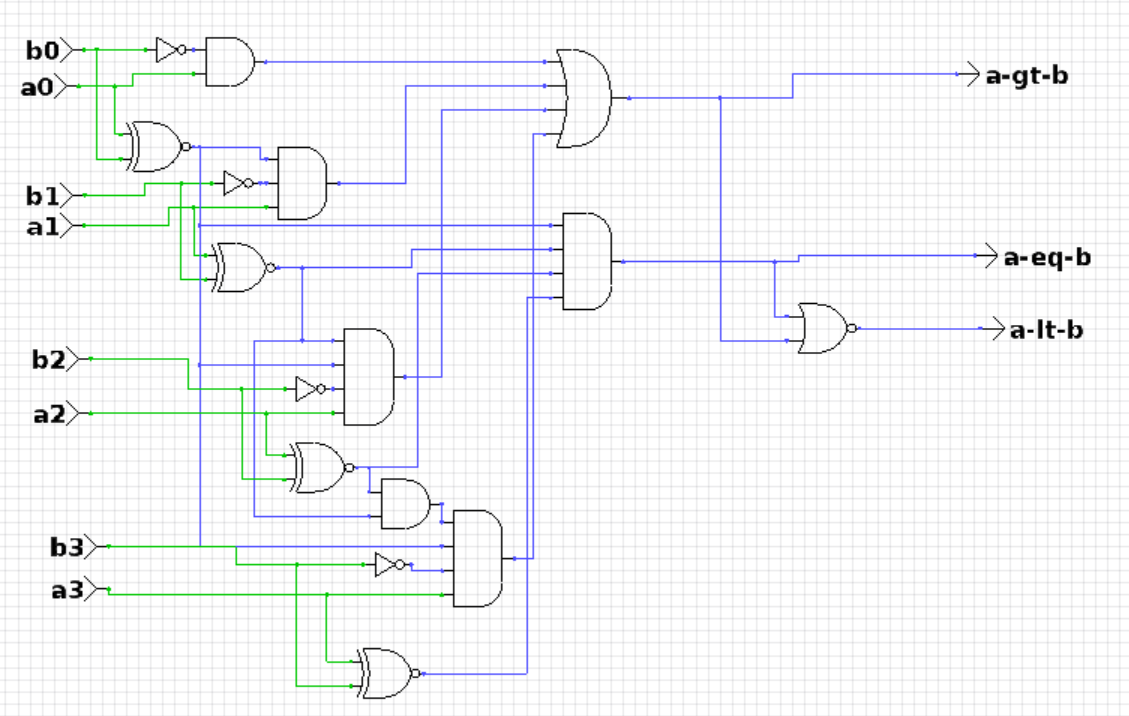
\includegraphics[width=\columnwidth]{comparator.png}}%
}%
\end{figure}

\subsubsection{Defining a Functional Comparator}
In order to prove the correctness of this circuit using ACL2, we first needed to define our own model for the 3 functions of the comparator. Not that these functions assume the inputs are in little-endian order. 

\begin{lstlisting}
;; = relation for variable-length vectors 
(defun v-= (a b)
  (if (atom a)
      (atom b)
    (and (xnor (car a) (car b))
         (v-= (cdr a) (cdr b)))))

;; < relation for variable-length vectors
(defun v-< (a b)
  (if (atom a)
      nil
    (if (equal (cdr a) (cdr b))
        (and (not (car a)) (car b))
      (v-< (cdr a) (cdr b)))))

;; > relation for variable-length vectors
(defun v-> (a b)
  (v-< b a))
\end{lstlisting}

After we have defined a functional model that implements the functional output of a comparator, we can then leverage ACL2's reasoning system to check if the created model is correct. We can prove that these functions produce the correct output by converting the input bit vectors into natural numbers. The defthm declaration for the $<$ relation is shown below. The v-to-nat function was provided by Dr. Hunt. It converts a little-endian bit vector represented as a boolean list to a natural unsigned number. The induction hint to use the induct-hint-both function to define the schema of inductive steps simply tells the theorem prover to reduce both a and b to be the 
\lstinline{(cdr a)} and \lstinline{(cdr b)}. 

\begin{lstlisting}
(defthm v-to-nat-equal
  (implies (and (boolean-listp a)
                (boolean-listp b)
                (= (len a) (len b)))
           (equal (= (v-to-nat a)
                     (v-to-nat b))                   
                  (equal a b)))  
:hints (("Goal" :induct (induct-hint-both a b))))
  
(defthm v->-correct
  (implies (and (boolean-listp a)
                (boolean-listp b)
                (= (len a) (len b)))
           (iff (v-> a b)
                (> (v-to-nat a) (v-to-nat b)))))
\end{lstlisting}

After the previous theorems are verified and entered into the ACL2 logic, we can use them to verify the netlist that was generated from the first step. This accomplished by presenting the theorem prover with an equality relation that involves functions from the general model and the netlist we are trying to verify. 

\begin{lstlisting}
(defthm comparator-netlist-compares-<
  (implies 
    (boolean-listp '(a0 a1 a2 a3 b0 b1 b2 b3))
    (equal (v-< '(a0 a1 a2 a3) '(b0 b1 b2 b3))
           (nth 2 (4-bit-comparator-netlist 
                    a0 a1 a2 a3 b0 b1 b2 b3)))))
\end{lstlisting}

The above statement tells the story for the $<$ relation, as the \lstinline{defthm} statements for the other functions are almost identical. This pattern of explicitly defining the variables to be used in the proof in the hypothesis of the theorem will be carried over to each of the different methods used to prove correctness of these these circuits which have a finite definition.

\section{The Carry Look-ahead Adder}
As a more interesting example, consider a carry-lookahead adder. A carry-lookahead adder is a type of logical adder which computes addition in logarithmic time. In traditional ripple carry adders, each adder must wait for the output carry to be propagated from the previous adder unit, resulting in a computation that is linear in time. Lookahead units compute $N-1$ carry bits based on the values of a propagate and generate bit from each of the $N$ adders that are connected as masters to the lookahead.

The Texas Instruments TTL\cite{TTL} defines two modules which can be used to create such an adder:
\begin{itemize}
\item SN74AS181A -- an ALU circuit with support for addition of two 4-bit vectors
\item SN74AS182 -- a look-ahead carry circuit for performing addition in logarithmic time
\end{itemize}

\footnote{The arrows connecting the carries from the lookahead on the bottom are pointing in the wrong direction. This is a mistake in the TTL.}Figure 2 shows an excerpt of such a system with 16 SN74AS181A modules functioning as adders with 5 SN74AS182 lookahead units.

\begin{figure}[ht!]
  \caption{A 64-bit carry look-ahead adder from the TTL \cite{TTL}}
  {%
\setlength{\fboxsep}{0pt}%
\setlength{\fboxrule}{1pt}%
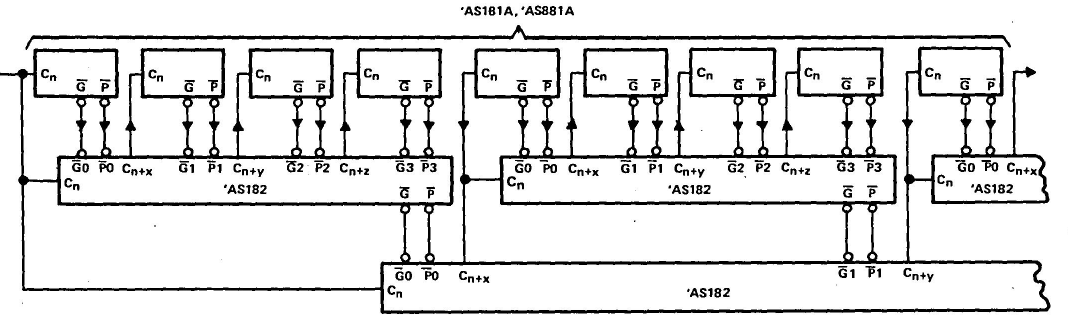
\includegraphics[width=\columnwidth]{lookahead.png}%
}%
\end{figure}

An interesting property of the lookahead adder exists in the mutual dependency between the lookahead unit and the adders. Appendix A.2 and A.3 show the gate diagram of the '181 and '182 modules. Looking at these diagrams and observing how these modules connect together illustrates that each carry produced by the '182 requires the values for the propagate and generate bits for the previous adders be present, and the adders need the carry produced by the lookahead to perform their logical function. For our simple netlist model, this poses a problem. Since the model of the circuit is embedded into ACL2 logic itself, the ACL2 evaluator has no way of knowing how to split up the complete circuit to complete the computation. There are 2 approaches of solving this problem:
\begin{itemize}
\item Evaluate the '182 module repeatedly, being careful to supply values to unused inputs which will not affect the desired outputs of the module
\item Flatten the circuit, effectively isolating the functionality of each output in the '182
\end{itemize}

There is another way of modeling the circuits which hides these problems associated with evaluation. By representing the model as data instead of ACL2 logic directly, an evaluator can be written which gives functional meaning to the data and provides a nice abstraction to the user. This approach is discussed later.

\subsection{The SN74AS181}
When the '181 is in $add$ mode, it offers 7 inputs and 11 outputs that are relevant for addition. The '181 accepts 2 4-bit input bit-vectors and an input carry. The output consists of an output carry bit, 4 bits comprising the first input vector, 4 bits comprising the second input vector, a propagate bit, and a generate bit. The '181 was already defined by Dr. Hunt, as well as a generic adder for performing vector addition. All verification was done with $S=1001$ (add) and $m=0$ (active-low data). 
  
%------------------------------------------------
\phantomsection
\section*{Acknowledgments} % The \section*{} command stops section numbering

\addcontentsline{toc}{section}{Acknowledgments} % Adds this section to the table of contents

So long and thanks for all the fish.
\cite{Conway2000}
%----------------------------------------------------------------------------------------
%	REFERENCE LIST
%----------------------------------------------------------------------------------------

\bibliographystyle{plain}
\bibliography{bibpage}

%----------------------------------------------------------------------------------------

\appendix
\section*{Appendix}
\section{Figures}
\subsection*{Output of CircuitToAcl2 given XML of circuit defined in Figure 1}
\begin{lstlisting}
(defun 4-bit-comparator-netlist (a0 a1 a2 a3 b0 b1 b2 b3)   
(let* (          
       (w12 (xnor a0 b0))          
       (w19 (not b3))          
       (w1 (xnor a1 b1))          
       (w14 (not b2))          
       (w7 (not b1))          
       (w3 (not b0))          
       (w17 (xnor a2 b2))          
       (w26 (xnor a3 b3))          
       (w18 (and w1 w12 w14 a2))          
       (w10 (and w3 a0))          
       (w2 (and w17 w1))          
       (w27 (and w12 w1 w17 w26))          
       (w11 (and w12 w7 a1))          
       (w25 (and w2 w12 w19 a3))          
       (w28 (or w10 w11 w18 w25))          
       (w29 (nor w27 w28))          
       (a-eq-b w27)          
       (a-gt-b w28)          
       (a-lt-b w29))     
  (list a-eq-b a-gt-b a-lt-b)))
\end{lstlisting}

\subsection*{The SN74AS181 Diagram from the TTL \cite{TTL}}
\end{document}